\ylDisplay{Must kast} % Ülesande nimi
{EFO žürii} % Autor
{piirkonnavoor} % Voor
{2019} % Aasta
{P 6} % Ülesande nr.
{2} % Raskustase
{
% Teema: Elektriõpetus

\ifStatement
Kahe väljundklemmiga mustas kastis on mingil viisil ühendatud kolm ühesuguse takistusega takistit ja üks lüliti. Kui mõõta väljundklemmide vahelist takistust, siis sõltuvalt lüliti asendist on tulemuseks kas $15$ $\Omega$ või $20$ $\Omega$. Leidke, kuidas on ühendatud takistid ja lüliti ning milline on takisti takistus.
\fi

\ifHint
Kuna lüliti asend muudab takistust, siis peab lüliti ühendama süsteemist välja vähemalt ühe takisti nii, et süsteemist läheb vool ikkagi läbi.
\fi


\ifSolution
Kuna lüliti asend muudab takistust, siis peab lüliti ühendama süsteemist välja vähemalt ühe takisti nii, et süsteemist läheb vool ikkagi läbi. Seega peab süsteemis esinema rööpühendus. Üheks võimaluseks on ühendada takistid joonisel näidatud viisil. Kui lüliti on avatud, ülemisest takistist vool läbi ei lähe ning kaks alumist takistit on omavahel ühendatud jadamisi. Kui lüliti on suletud, on parempoolsed takistid ühendatud rööbiti. Kuna süsteemi takistused peavad olema sõltuvalt lüliti asendist $15$ $\Omega$ ja $20$ $\Omega$, siis peab olema ühe takisti takistus $10$ $\Omega$. Seega, kui lüliti on avatud, on süsteemi kogutakistus $R_{lahti} = R + R = 20$ $\Omega$. Kui lüliti on suletud, on rööpühenduse kogutakistus $\frac{1}{R_{rööp}} = \frac{1}{R} + \frac{1}{R}$ $\Rightarrow$ $R_{rööp} = 5$ $\Omega$. Süsteemi kogutakistus on seega suletud lüliti korral $R_{kinni} = R + R_{rööp} = 15$ $\Omega$.
\begin{center}
	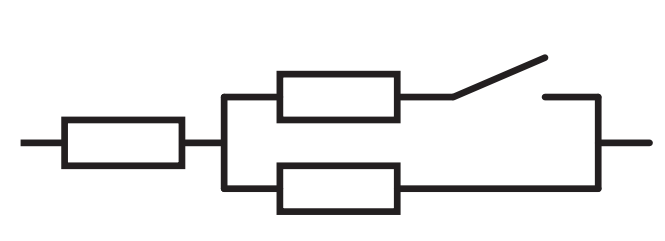
\includegraphics[width=0.5\linewidth]{2019-v2p-06-lah.png}
\end{center}
\fi
}